\section{Introduction}\label{sec:introduction}

Software bugs are an inevitable part of the development process. Bugs can lead to security problems, loss of company profit, and in the worst case, even fatal accidents~\cite{wong2017more}. For these reasons, bugs need to be swiftly fixed, which requires choosing the most appropriate developer. The problem of finding such a developer for a particular bug is called \textit{bug triage}~\cite{Anvik2006WhoSF}.

The developer who should fix the bug can be assigned manually, however, such an approach has several significant disadvantages. Firstly, it is tedious and time-consuming work, and the situation gets more and more complicated as the number of developers grows. In large companies, hundreds of bug reports are received every day, which makes manual developer assignment very difficult if not impossible. For example, 333,371 bugs were reported for the Eclipse IDE from October 2001 to December 2010, averaging at about 100 bugs every day~\cite{Xuan2012DeveloperPI}. Secondly, it is important to assign the most suitable developer right from the start to reduce the time of bug fixing~\cite{Anvik2006WhoSF}. Otherwise, the error gets reassigned from one developer to another~\cite{Jeong2009ImprovingBT}, and as a result, the time of each developer in such a chain is wasted, while the error remains in the system longer, which can be critical. 

A large number of approaches have been proposed to solve the bug triage problem automatically. Existing models can be roughly divided into three groups: based on heuristics~\cite{Tian2016LearningTR, Tamrawi2011FuzzySA, Shokripour2015ATA, Hu2014EffectiveBT}, based on classic machine learning~\cite{Naguib2013BugRA, Xia2017ImprovingAB, sarkar2019improving}, and based on deep learning (DL)~\cite{Lee2017ApplyingDL, Guo2020DeveloperAM, Mani2019DeepTriageET, Xi2019BugTB}. The works of Guo et al.~\cite{Guo2020DeveloperAM} and Mani et al.~\cite{Mani2019DeepTriageET} demonstrated that deep learning helps with the task of assigning a developer better than other approaches.  This is to be expected, since the bug triage task is based on natural language processing, where deep learning shows promising results~\cite{Wolf2020TransformersSN}. An additional advantage of deep learning algorithms is that they do not require sophisticated feature extraction methods~\cite{Schmidhuber2015DeepLI}.

However, it should be noted that bugs can be reported in different forms. For example, in a bug tracking system, errors are usually present in the form of a bug report: a name, a small description in some natural language, and some additional meta information (the date the error was introduced, priority, severity, etc.). To the best of our knowledge, all the existing solutions are based on working with this kind of error representation. At the same time, errors can also come in the form of \textit{stack traces}: sequences of function calls (called \textit{frames}) that lead to an error in the system. Developers commonly use stack traces during debugging, and users can usually see a stack trace displayed as part of an error message. Stack traces help to solve the bug localization problem~\cite{Wong2014BoostingBF, Moreno2014OnTU, Youm2015BugLB} and the bug report deduplication problem~\cite{Dang2012ReBucketAM, Sabor2017DURFEXAF, Khvorov2021S3MSS}. The example of a single stack frame is presented in \Cref{fig:introduction-frame-example}. 

\begin{figure}[h]
    \centering
    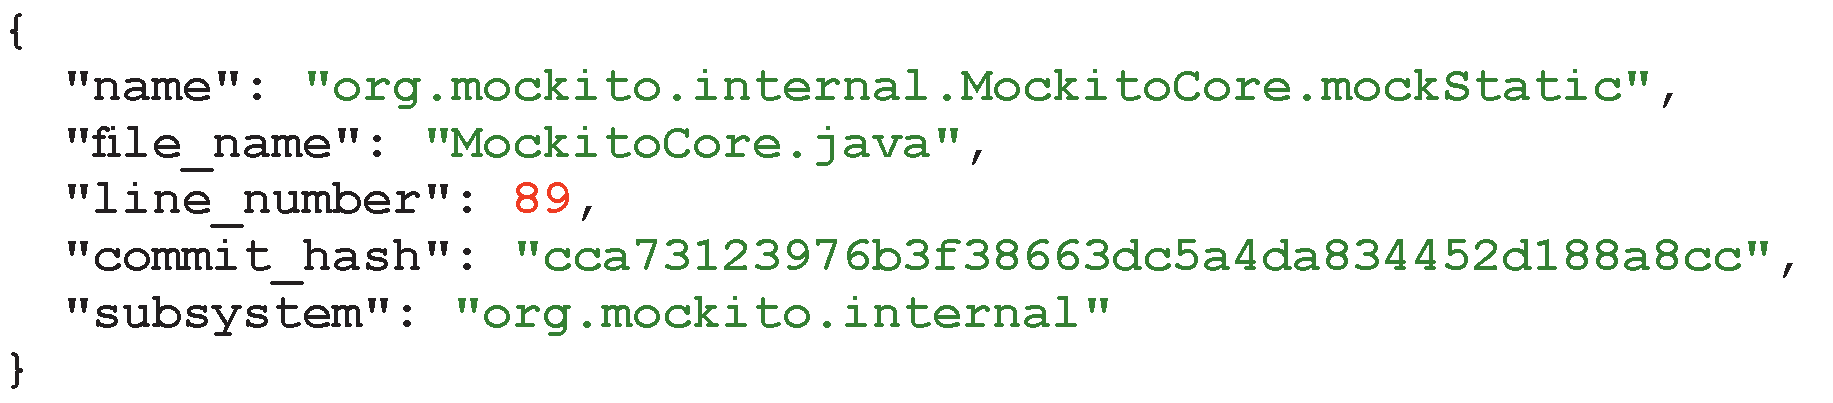
\includegraphics[width=\columnwidth]{figures/01-introduction/frame-example.pdf}
    \vspace{-0.5cm}
    \caption{An example of a stack frame. The frame consists of the name of the function that led to the error, as well as various information about it.}
    \label{fig:introduction-frame-example}
\end{figure}

Stack traces are a data source that is often easy to obtain: most modern software systems are able to automatically send back stack traces of the error that has occurred. In such a setting, predicting the assignee by the textual description of the error would require labeling all the error reports, which is almost impossible since the number of such reports per day could be enormous. Another important reason to process stack traces automatically is that they are more complicated to analyze manually by people who did not participate in the development of a particular system component, since the information is presented in a rather raw form. Thus, a new approach is needed that solves the bug triage problem for the case where only the stack trace information is available.

Another important limitation of the existing approaches is that they consider the bug triage task as a classification problem. The classification setting might not be the best choice in practice, since the set of classes (developers) can change over time: developers can leave and join the team responsible for the product of even the company itself. 

To the best of our knowledge, no one has previously suggested using bug stack traces as the main source of information for the bug triage problem. In this work, we strive to fill this gap in research to support working with the systems where stack traces are the primary type of data. To that end, we collected two datasets of real-world bug stack traces from JetBrains,\footnote{JetBrains: \url{https://www.jetbrains.com/}} the developer of a wide array of software products including IntelliJ-based IDEs. The larger dataset contains 11,139 stack traces, however, it contains proprietary company code, so we also curate the second dataset --- a smaller public subset of the first one that contains 3,361 stack traces that we release for researchers and practitioners. The datasets consist of a labeled set of bug reports and annotations from the version control system (developer IDs and timestamps) that we apply to improve the quality of our model.

We propose a new approach to solve the bug assignee prediction problem based on stack traces --- a DL-based ranking model called \textit{DapStep} (an RNN ranking model with manual frame-based \& stack-based features). We compared the proposed model with existing approaches adapted for stack trace processing. The proposed model shows Acc@1 of 0.34 and MRR of 0.43 on the public dataset and Acc@1 of 0.60 and MRR of 0.70 on the private dataset.

The main contributions of this paper are as follows:
\begin{itemize}
    \item We propose bug stack traces as a self-sufficient source of information for the assignee prediction task and carry out the first study in comparing various approaches in this setting.
    \item We introduce two bug triage ranking models based on recurrent neural networks (RNN) with the attention mechanism and convolutional neural networks (CNN). The models outperform the existing classification approaches by
    15--20 percentage points on the public dataset, and 17--18 percentage points on the private dataset.
    \item We publish the source code of all the studied models, as well as the public dataset, for future researchers and practitioners: \url{https://github.com/Sushentsev/DapStep}.
\end{itemize}

The remaining sections of this paper are organized as follows. \Cref{sec:related-work} provides a brief overview of existing solutions, and in \Cref{sec:approach}, we propose a new deep learning solution. We evaluate our approach in \Cref{sec:evaluation}, followed by a discussion of the threats to validity in \Cref{sec:threats-to-validity}. Finally, \Cref{sec:conclusion} summarizes the results of the paper.